% !TEX root =  ../main_manuscript.tex 
\section{Demonstration of Personalized Schedules}
\label{sec:results}
We return to the prostate cancer active surveillance dataset, PRIAS, described in Section~\ref{sec:introduction}. The clinical data consists of longitudinal PSA (continuous; ng/mL) and DRE (binary; tumor palpable or not) measurements (Section~\ref{sec:introduction}), patient age at baseline, history of biopsies, and interval-censored times of cancer progression. The event of interest is cancer progression. We aim to use the accumulated clinical data to build joint models that can be utilized for creating personalized biopsy schedules in future PRIAS patients. 

The current PRIAS protocol for biopsies is fixed biopsies at year one, four, seven, and ten of follow-up, and every five years after that. Additional yearly biopsies are scheduled if a patient's PSA doubling-time~\citep{bokhorst2015compliance} is high. The PSA is measured as per a fixed schedule, quarterly for the first two years, and semi-annually after that. The DRE is also measured semi-annually.

\subsection{Fitting the Joint Model to the PRIAS Dataset}
We first fit a joint model to the accumulated clinical data, with $\log_2(\mbox{PSA} + 1)$ transformed PSA~\citep{lin2000latent,pearson1994mixed}, and DRE as longitudinal measurements, and cancer progression as the event. In the PSA linear mixed-effects sub-model, we utilize B-splines~\citep{de1978practical} to allow non-linearly evolution of PSA over follow-up. For DRE, we utilize a logistic mixed-effects sub-model. To link the longitudinal sub-models for the PSA and DRE with the relative-risk sub-model for cancer progression, we include three features of the longitudinal outcomes in the relative-risk sub-model. Specifically, the hazard of cancer progression at time $t$ depends on the fitted instantaneous $\log_2(\mbox{PSA} + 1)$ value at time $t$, the estimated instantaneous $\log_2(\mbox{PSA} + 1)$ velocity at $t$, and fitted log-odds of having a DRE indicating a palpable tumor at $t$. We estimated the parameters of our model under the Bayesian framework using the R package \textbf{JMbayes}~\citep{rizopoulosJMbayes}. The resulting parameter estimates showed that $\log_2(\mbox{PSA} + 1)$ velocity was the strongest indicator of cancer progression (adjustedhazard ratio...bla bla). The detailed specification of the joint model and the resulting parameter estimates are in Web-Appendix.

\subsection{Personalized Schedules for a Demonstration Patient}
We utilize the fitted joint model to schedule biopsies in a real PRIAS patient (Figure~\ref{fig:demo_schedule}). To this end, in line with the protocols of most prostate cancer surveillance cohorts, we first schedule a compulsory biopsy at year one of follow-up~\citep{nieboer2018active}. This biopsy promises early detection of progression for patients misdiagnosed as low-grade cancer patients or patients who chose surveillance despite having a higher grade at diagnosis. We also maintain a recommended minimum gap of one year between consecutive biopsies~\citep{bokhorst2016decade}. Consequently, we schedule personalized biopsies starting from year two. The added benefit of this approach is that due to the clinical data accumulated over two years, we can make reasonably accurate predictions of the cumulative-risk of progression. The follow-up period of PRIAS is limited currently. Hence, we are able to estimate the cumulative-risk of progression (Equation~\ref{eq:cumulative_risk}) and subsequently schedule biopsies only until year ten of follow-up.

In Figure~\ref{fig:demo_schedule} we can see

\begin{figure}
\centerline{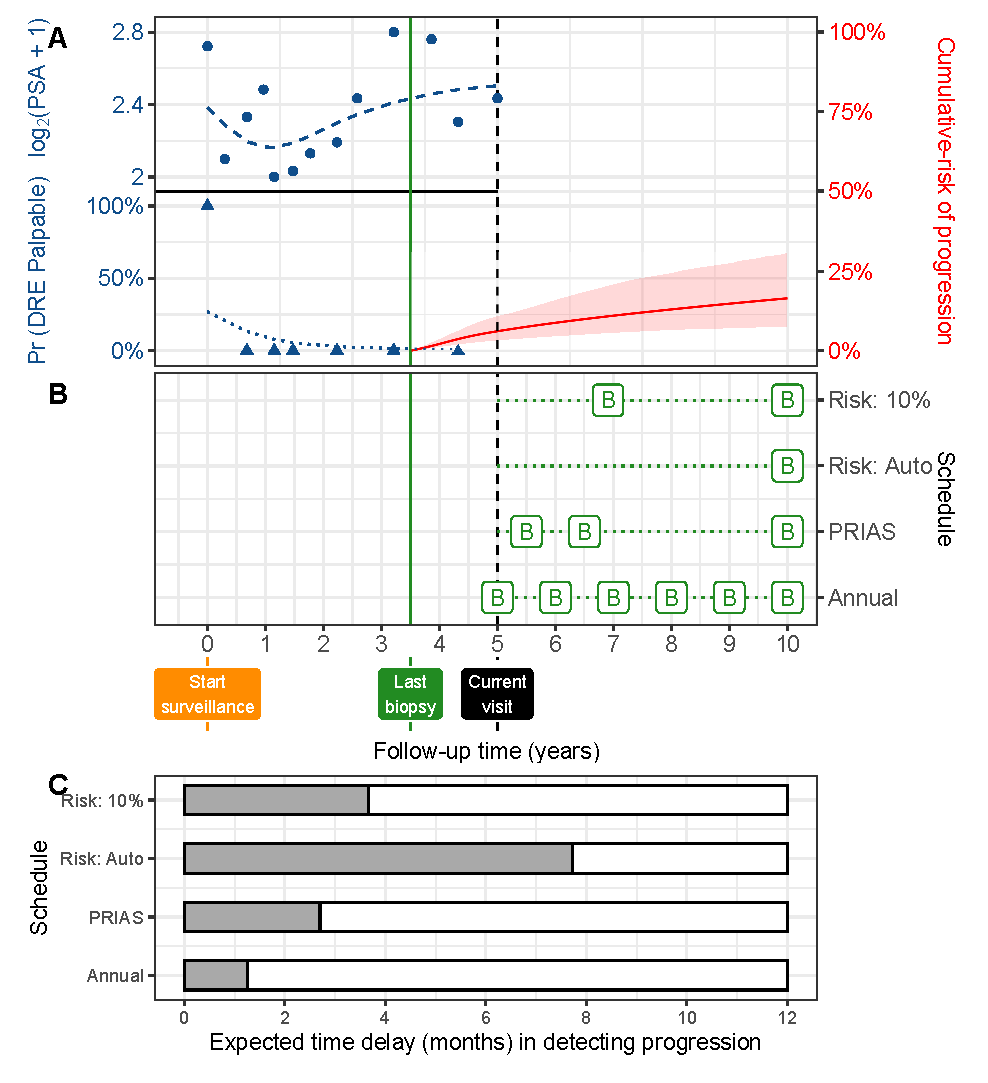
\includegraphics{images/demo_schedule.eps}}
\caption{\textbf{Demonstration } as more patient data is gathered. A single longitudinal outcome, namely, a continuous biomarker of disease progression is used for illustration. \textbf{Panels~A,B~and~C:} are ordered by the time of the current visit (dashed vertical black line) of a new patient. At each of these visits, we combine the accumulated longitudinal measurements (shown in blue), and last time of negative invasive test (solid vertical green line) to obtain the updated cumulative risk profile (shown in red) of the patient. All values are illustrative.} 
\label{fig:demo_schedule}
\end{figure}